\subsection{Example: \(4\pi\)-Periodic Soliton and Spin-1/2}
  \label{subsec:4pi_soliton}

  To illustrate how a \(4\pi\)
  -periodic soliton can represent a spin-1/2 particle, consider a 1D soliton solution for the \(\chi\)
  field with a phase twist. Let \(\chi(x)\) be a complex field defined as:

  \[
    \chi(x) = \eta \tanh(\kappa x) e^{i \theta(x)},
  \]

  where \(\eta\) is the amplitude, \(\kappa\) determines the soliton's width, and \(\theta(x)\)
  is the phase. For a spin-1/2 particle, the phase \(\theta(x)\) must satisfy:

  \[
    \theta(x + 2\pi) = \theta(x) + \pi, \quad \theta(x + 4\pi) = \theta(x) + 2\pi.
  \]

  This \(4\pi\)-periodicity reflects the double-valuedness of spinors under rotations.

  \subsubsection{Explicit Construction of a \(4\pi\)-Periodic Soliton}

    Define the phase \(\theta(x)\) as:

    \[
      \theta(x) = \frac{x}{2},
    \]

    so that a full rotation \(x \to x + 4\pi\) returns the phase to its original value:

    \[
      \theta(x + 4\pi) = \frac{x + 4\pi}{2} = \theta(x) + 2\pi.
    \]

    The soliton solution is then:

    \[
      \chi(x) = \eta \tanh(\kappa x) e^{i x/2}.
    \]

    This soliton has the following properties:
    \begin{itemize}
      \item It is localized around \(x = 0\), with \(\chi(x) \to 0\) as \(|x| \to \infty\).
      \item The phase winds by \(\pi\) as \(x\) goes from \(-\infty\) to \(+\infty\), but a full \(2\pi\)
      rotation of the soliton requires \(x \to x + 4\pi\), reflecting the spin-1/2 nature.
    \end{itemize}

  \subsubsection{Topological Interpretation}

    The \(4\pi\)-periodicity of the soliton is a manifestation of its \textbf{topological winding number}
    . For a closed loop in space, the phase change \(\Delta \theta\) is given by:

    \[
      \Delta \theta = \oint \nabla \theta \cdot d\mathbf{l} = 2\pi n,
    \]

    where \(n\) is the winding number. For a spin-1/2 particle, the effective winding is \(n = 1/2\)
    , but since the phase must be single-valued in space, the soliton must traverse the loop twice to return to
    its original state, hence the \(4\pi\)-periodicity.

  \subsubsection{Connection to Quantum Statistics}

    The \(4\pi\)-periodicity of the soliton directly implies that it obeys \textbf{fermionic statistics}:
    \begin{itemize}
      \item Under a \(2\pi\) rotation, the wavefunction of the soliton acquires a phase of \(e^{i\pi} = -1\)
      , which is the hallmark of a fermion.
      \item This explains the \textbf{Pauli exclusion principle}
      : two identical solitons cannot occupy the same state because their wavefunctions would interfere
      destructively due to the \(-1\) phase factor.
    \end{itemize}

    \begin{figure}[h]
      \centering
      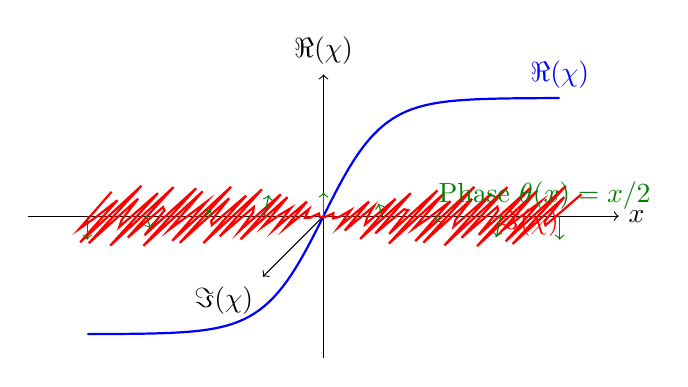
\begin{tikzpicture}[x=1.5cm, y=1.5cm]
        % Axes
        \draw[->] (-2.5,0) -- (2.5,0) node[right] {$x$};
        \draw[->] (0,-1.2) -- (0,1.2) node[above] {$\Re(\chi)$};
        \draw[->] (0,0) -- (0,0,2) node[below left] {$\Im(\chi)$};

        % Real part of chi
        \draw[thick, blue, domain=-2:2, samples=100] plot (\x, {tanh(2*\x)}, 0);
        \node[blue, above] at (2, 1, 0) {$\Re(\chi)$};

        % Imaginary part of chi
        \draw[thick, red, domain=-2:2, samples=100] plot (\x, 0, {tanh(2*\x)*sin(deg(90*\x))});
        \node[red, above] at (2, 0, 1) {$\Im(\chi)$};

        % Phase arrows
        \foreach \x in {-2, -1.5, ..., 2} {
          \pgfmathsetmacro{\phase}{90*\x}
          \draw[green!50!black, ->] (\x, 0, 0) -- (\x, {0.2*cos(\phase)}, {0.2*sin(\phase)});
        }
        \node[green!50!black] at (2, 0.3, 0.5) {Phase $\theta(x) = x/2$};
      \end{tikzpicture}
      \caption{
        Visualization of a \(4\pi\)-periodic soliton representing a spin-1/2 particle.
        The real part \(\Re(\chi)\) (blue) and imaginary part \(\Im(\chi)\) (red) of the \(\chi\) field are shown,
        along with the local phase (green arrows).
        The phase winds by \(\pi\) over the spatial extent of the soliton, but a full \(2\pi\)
        rotation of the soliton requires a \(4\pi\) change in phase, reflecting its fermionic nature.
      }
      \label{fig:4pi_soliton}
    \end{figure}
